The network metering with Zabbix is not only used for network managing  decisions. It is also possible for each user of the \textit{Smart Filesystem} to get informations concerning his used energy and his created costs.
\subsection{A Cost Request}
 The idea is, that each user can go on a website and requests for his account a special time frame. This procedure is shown in figure \ref{akt}.
 \begin{figure}
 \centering
 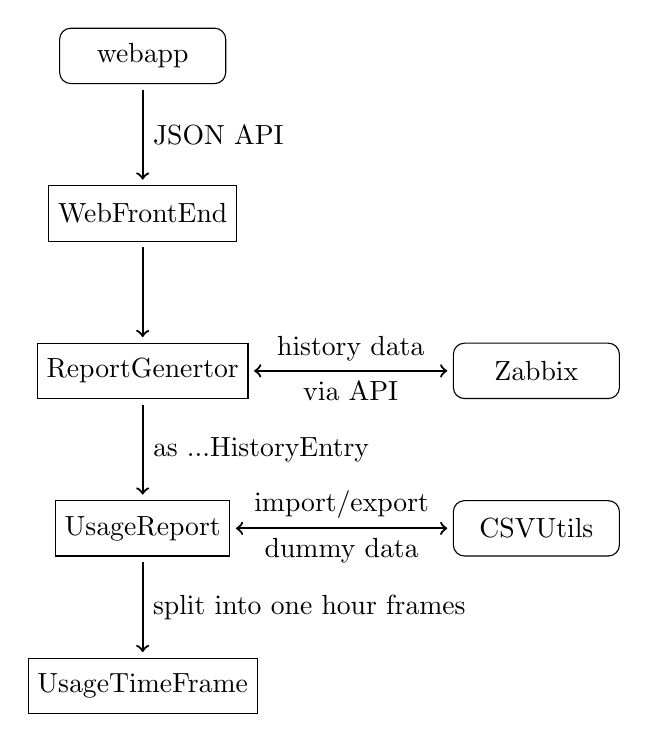
\begin{tikzpicture}
    \tikzset{
        external/.style = {
            rectangle, rounded corners, draw=black,
            minimum width=6em, minimum height=2em, text centered, node distance=5cm
        },
        internal/.style = {
            rectangle, draw=black,
            minimum width=6em, minimum height=2em, text centered, node distance=2cm
        },
        edge/.style = {
            ->, thick, shorten <= 2pt, shorten >= 2pt
        },
        dotted box/.style = {
            rectangle, draw = black, rounded corners, dashed, inner sep=3pt
        }
    };

	\node[internal] (generator) {ReportGenertor};
	\node[internal] (web) [above of = generator] {WebFrontEnd};
	\node[external, node distance = 2cm] (webapp) [above of = web] {webapp};
	\node[external] (zabbix) [right of = generator]  {Zabbix};
	\node[internal] (report) [below of = generator] {UsageReport};
	\node[external] (csv) [right of = report] {CSVUtils};
	\node[internal] (frame) [below of = report]{UsageTimeFrame};

	\draw[edge] (webapp) -- (web) node [midway, right] {JSON API};
	\draw[edge] (web) -- (generator);
	\draw[edge, <->] (generator) -- (zabbix)
		node [midway, above] {history data}
		node [midway, below] {via API};
	
	\draw[edge, <->] (report) -- (csv) 
		node [midway, above] {import/export} 
		node [midway, below] {dummy data};
	
	\draw[edge] (generator) -- (report)
		node [midway, right] {as ...HistoryEntry};
	\draw[edge] (report) -- (frame) 
		node [midway, right] {split into one hour frames};
\end{tikzpicture}
 \caption{Activity diagram of a user's cost request}
 \label{akt}
 \end{figure}


 The request goes to the "ReportGenerator" which uses the account of the user and the given time frame to create an API request for Zabbix. Zabbix gets all information about the user in the given time frame from its database and sends it back to the ReportGenerator. Now these information will be packed as so called "HistoryEntries" and forwarded to an instance of the "UsageReport" class. 
 
 This instance can import or export the data as files or starts the price calculation. To do that the UsageReport splits the data in one hour frames. This is possible because Zabbix stores for each data the time as well. These calculations will be made by the "UsageTimeFrame". After that the system can tell the user how much he has to pay for the given time by listing the usage in one hour parts.
 
 \subsection{Calculation of the price} 
 The basic idea of the price concept is that the owners of the \textit{Smart Filesystem} do not have to pay for the maintenance of the system. Every user has pay a part of the energy usage if the severs run in idle mode. The part depends on how much data the user has stored in the system. Moreover the user has to pay for his traffic. It should be noticed that this basic idea, which was made by the team. It can't work if just a few persons uses the system. On the other hand the idea of distributed file systems is that a lot of people use them. But it was not possibly to test that concept because there simply were not that much test users. 
 
 If we want to compute the price for each user in an hour, the first thing to do is to extend the data from Zabbix. Firstly Zabbix stores energy usage of each sever every two seconds. Secondly, if there is a traffic flow, Zabbix will store information about that every five seconds. And last but not least Zabbix stores the used data of each user if it changes. Imagine a situation where user \textit{u} transfers 100 megabytes in 10 seconds to the \textit{Asok05} server. Then the information created by Zabbix looks like the table \ref{tb1}. 
\begin{table}
\centering
\caption{Generated data from Zabbix of user \textit{u}}
\begin{tabular}{|c|c|c|c|}
 \hline Time in $s$ & Data in $MB$ & Traffic in $MB/s$ & Energy in $W$ \\ 
  \hline 0 & 3000 & 0 & 400 \\ 
 \hline 1 & - & 10 & - \\ 
 \hline 2 & - & - & 450 \\ 
 \hline 3 & - & - & -\\ 
 \hline 4 & - & - & 450 \\ 
 \hline 5 & - & - & - \\
 \hline 6 & - & 10 & 445 \\ 
 \hline 7 & - & - & -\\ 
 \hline 8 & - & - & 450 \\ 
 \hline 9 & - & - & - \\  
 \hline 10 & - & - & 430 \\
  \hline 11 & - & 10 & - \\
 \hline 12 & 3100 & 0 & 400 \\  
 \hline 
 \end{tabular}
 \label{tb1} 
 \end{table}
 
 To get clear information when a flow starts and when a flow stops, Floodlight sends at the start and the end of a flow a zero to Zabbix. The given information is not enough compute a clear price for each user. So the next step is to complete the table for each user. For every empty energy entry the system takes the next known value. For the data usage the system takes the last known value. The same goes for traffic. So after that the table looks like table \ref{tb2}.
 
 
 \begin{table}
 \centering
 \caption{Extended Data of user \textit{u}}
 \begin{tabular}{|c|c|c|c|}
  \hline Time in s & Data in $MB$ & Traffic in $MB/s$ & Energy in $W$ \\ 
   \hline 0 & 3000 & 0 & 400 \\ 
  \hline 1 & 3000 & 10 & 450 \\ 
  \hline 2 & 3000 & 10 & 450 \\ 
  \hline 3 & 3000 & 10 & 450\\ 
  \hline 4 & 3000 & 10 & 450 \\ 
  \hline 5 & 3000 & 10 & 445 \\
  \hline 6 & 3000 & 10 & 445 \\ 
  \hline 7 & 3000 & 10 & 450\\ 
  \hline 8 & 3000 & 10 & 450 \\ 
  \hline 9 & 3000 & 10 & 430 \\  
  \hline 10 & 3000 & 10 & 430 \\
   \hline 11 & 3000 & 10 & 400 \\
  \hline 12 & 3100 & 0 & 400 \\  
  \hline 
  \end{tabular}
  \label{tb2} 
  \end{table}
  
  This extended table will be created for each user, each server and for each hour in the given time frame. If there is user data synchronization between the servers, it will identified as "internal traffic" and will be accounted for a user on the system which does the synchronization. After that, the system can compute a price for each user in each second of an hour. After that it sums up the prices and computes the mean value. Then we have the costs for each user and for each system. The last step is to sum up the mean values for each system to get the total costs for a user in an hour.
  
  Computing the price for second must be separated in two different situations. The question is: "Does the user create traffic in this second?":
  \begin{enumerate}
	\item
	If not, the system will compute the ratio of used data storage to overall used data storage and multiplies it by the power consumption of the server in idle mode.
	\item
	If the user does create traffic it will do the same as in step one. Moreover it will compute the ratio of user traffic to all user traffic to this server and multiplies it with the needed energy in this second deducing the idle energy consumption.
  \end{enumerate}
  
  \subsection{Example}
     For instance the idle energie consumption of \textit{Asok05} is $400\ W$. Moreover say that the overall user storage in the moment is $3\ TB$ and the energy price is $21\ cent$ per $KW/h$. So for second \textit{0} the user has to pay:
    
    $$(\frac{3000}{3000000} \cdot 400) = 0.4\ W $$
    
    Let's say in the 5th second there are two more users which create traffic of each 10 MB/s. So the used energy of our user is:
    
     $$(\frac{3000}{3000000} \cdot 400) + (\frac{10}{30} \cdot (450 - 400))  \approx 0.4 + 17 \approx 17.4\ W $$
           
  	This is how the system computes the energy for each second. The next step is to sum up these values. Imagine that the user did not create any more traffic in this hour. Then we have approximately:
  	
  	$$ 3590 \cdot 0.4\ W + 10 \cdot 17\ W \approx 1436 + 170 \approx 1606\ W$$
  	
  	This means the user has a mean energy usage of $1606 / 3600 \approx 0.45\ W/h$. If we multiplies that with current energy price of $21\ cent$ per $KW/h$, the user has tp pay $ 0.00045\ KW/h \cdot 21\ \frac{cent}{KW/h} \approx 0.01\ cent$ for this hour.
  	
  	Now the system sums up this prices of each server and returns the overall price for the user in this hour.  